\chapter{Implementación de la PCB\label{sec:Implementacion_PCB}}

En el diseño e implementación de la \acrshort{PCB} es muy importante tener presente que cualquier fallo a nivel de hardware supone una gran pérdida de tiempo y, por lo tanto, dinero. Desde que el diseño es terminado y se manda a producir la placa hasta que esta se recibe transcurre una media de dos semanas . Perder esa cantidad de tiempo por un fallo de diseño a nivel docente supone, en el peor de los casos, no entregar el proyecto en la fecha acordada pero a nivel empresarial puede significar perder la exclusividad del diseño cuando se compite con otras compañías. 

Las revisiones manuales permiten evitar ciertos errores pero una buena herramienta bien configurada contribuye a prevenir dichos errores desde el principio. Como ya se ha mencionado en el capítulo \ref{sec:Diseno}, para la realización de este proyecto se ha utilizado la herramienta KiCad, no sólo por ser Software Libre sino porque presenta ciertas características muy interesantes:
\begin{itemize}
\item \textbf{Entorno de desarrollo integrado:}
\\Desde la propia herramienta se pueden hacer los esquemáticos, definir los componenes y librerías e incluso diseñar y previsualizar la PCB.
\item \textbf{Multiplataforma:}
\\Disponible en Windows, Linux y Mac OS.
\item \textbf{Respaldado por una gran comunidad} 
\\Kicad tiene una gran comunidad que deja a disposición de los usuarios una documentación muy extensa.
\item \textbf{Constante desarrollo}
\\Se liberan actualizaciones con regularidad.
\end{itemize}

Tras instalar y configurar KiCad, al abrir la herramienta se carga un gestor de proyectos desde el que se puede gestionar un gran número de elementos. La figura \ref{fig:Front_end_Kicad} muestra a modo de ejemplo el estado de KiCad al final del proyecto.

\begin{figure} [h]
    \centering
    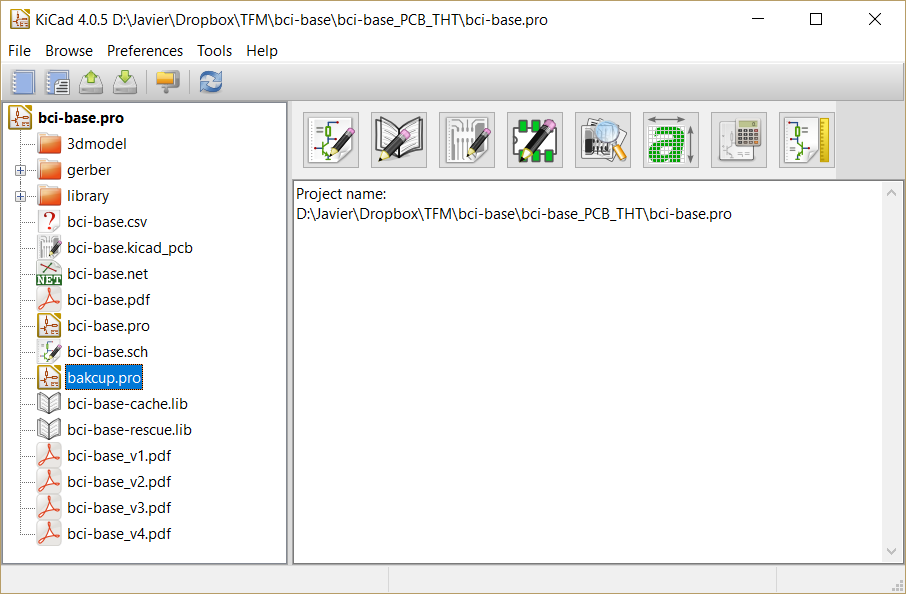
\includegraphics[width=13cm]{Front_end_Kicad}
    \caption{Gestor de proyectos de KiCad}
    \label{fig:Front_end_Kicad}
\end{figure}

Como se puede observar en la imagen, a la izquierda aparecen todos los archivos pertenecientes al proyecto mientras que en la parte superior hay un acceso directo a las distintas partes que componen KiCad (gestor de esquemáticos, librerías, modelos 3D, etc).

Durante la fase de diseño y realización del esquemático, cada componente fue seleccionado de entre los disponibles preinstalados con la herramienta. Aunque los componentes más comunes como son las resistencias o los condensadores se pueden encontrar sin problemas, para trabajar con otros componentes como el ESP ha sido necesario crear una librería propia. Más adelante, cuando las especificaciones de diseño se hayan definido, se enlazará el símbolo que representa cada componente con el elemento físico que estará presente en la \acrshort{PCB}, es decir, su \textit{footprint} y su modelo 3D.

\section{Limitaciones del fabricante\label{sec:ITEAD_PCB}}

El diseño de la PCB tiene ciertas restricciones, algunas impuestas por el propio diseño del circuito (tipo de componentes, número de pistas, tamaño final, etc.), otras, como las tratadas en esta sección, serán impuestas por el propio fabricante de \acrshort{PCB}s.

La mayoría de empresas fabricantes de PCBs del mercado dejan a disposición de sus clientes un listado de las limitaciones con las que cuentan, garantizando que cualquier diseño que se adecue a dichas especificaciones será impreso sin problemas. 

De entre las disponibles en Internet se seleccionó la compañía ITEAD por presentar una buena relación prestaciones/precio, haberse contratado sus servicios previamente y un buen tiempo desde la impresión hasta la recepción de la placa.

En su página web \cite{ITEAD_PCB_Limitations}, ITEAD ha preparado una tabla con un resumen de las características con las que se puede contar si se imprime una PCB en condiciones normales. Dicha tabla se recoge a continuación:

\begin{table} [H]
\centering
\begin{tabular}{|c|c|}
\hline 
\textbf{Característica} & \textbf{Valor} \\
\hline 
Layers &	1 - 4 \\
\hline 
Material & 	FR-4 \\
\hline 
Board Dimension (max) & 	380mm X380mm \\
\hline 
Board Dimension (min) &	10mm X10mm \\
\hline 
Outline Dimension Accuracy &  $\pm$0.2mm \\
\hline 
Board Thickness & 	0.40mm--2.0mm \\
\hline 
Board Thickness Tolerance &	 $\pm$10\% \\
\hline 
Dielectric Separation thickness &	0.075mm--5.00mm \\
\hline 
Conductor Width (min) &	0.15mm (Recommend>8mil) \\
\hline 
Conductor Space (min) &	0.15mm (Recommend>8mil) \\
\hline 
Outer Conductor thickness &	35um \\
\hline 
Inner Conductor thickness &	17um--100um \\
\hline 
Copper to Edge &	>0.3mm \\
\hline 
Plated Component &	 \multirow{2}{*}{0.3mm--6.30mm} \\
Plated via Diameter(Mechanical) & \\
\hline 
Plated Hole Diameter Tolerance(Mechanical) &	0.08mm \\
\hline 
Unplated Hole Diameter Tolerance &	0.05mm \\
\hline 
Hole Space(min) &	0.25mm \\
\hline 
Hole to Edge &	0.4mm \\
\hline 
Annular Ring(min) &	0.15mm \\
\hline 
Solder Resist Type & 	Photosensitive ink \\
\hline 
Solder Resist Color &	Black, Green, White, Blue, Yellow \\
\hline 
Solder Resist Clearance &	0.1mm \\
\hline 
Solder Resist Coverage &	0.1mm \\
\hline 
Plug Hole Diameter &	0.3mm--0.65mm \\
\hline 
Silkscreen line width (mim) &	6mil \\
\hline 
\end{tabular} 
\caption{Restricciones de ITEAD para la fabricación de una PCB}
\label{tab:ITEAD}
\end{table}

Aunque la lista de restricciones parece alta, la mayoría de ellas no supone un problema para un proyecto de estas dimensiones. Para comprobar si esta afirmación es correcta bastará con comprobar si la característica más restrictiva se cumple, es decir, comparar la separación mínima de los pads del módulo Bluetooth con la separación mínima entre conductores, denominada en la tabla \ref{tab:ITEAD} como \textit{Conductor Space}. De acuerdo a su \textit{datasheet}, la separación entre pines de este componente es de 9.84 mil (0.25 mm), valor muy superior a los 8 mil (0.2 mm) recomendados por el fabricante.
\clearpage
Adicionalmente, informan de que la utilización de \textit{Buried vias} y \textit{Blind vias} no es posible por el momento. En la figura \ref{fig:ITEAD_vias}, proporcionada por ITEAD en su página web, se ilustra como es cada tipo de vía.

\begin{figure} [h]
    \centering
    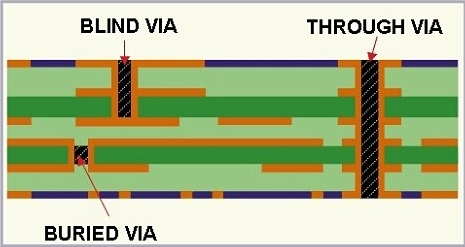
\includegraphics[width=10cm]{ITEAD_vias}
    \caption{Tipos de vías}
    \label{fig:ITEAD_vias}
\end{figure}

Con toda la información recopilada hasta el momento ya es posible configurar KiCad para forzar que dichas restricciones se cumplan en todo momento. El menú ``\textit{Design Rules}'' permite configurar estos parámetros (ver fig. \ref{fig:Design_rules_general}) así como realizar ciertos ajustes dependiendo de la función que tendrá cada pista ( ver fig. \ref{fig:Design_rules_especial}).

\begin{figure}[h]
  \begin{subfigure}[b]{8cm}
   	\centering
    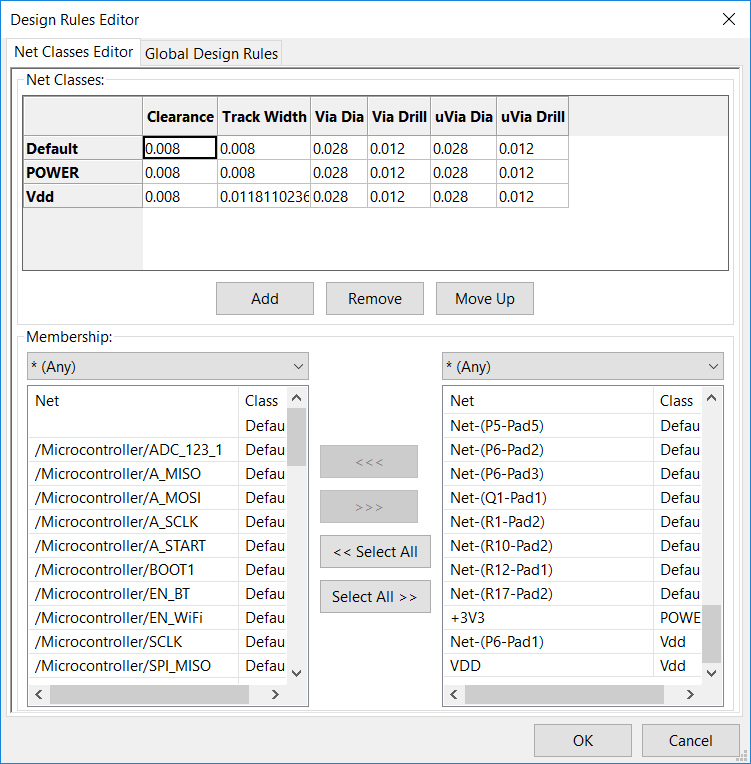
\includegraphics[width=8cm]{Design_rules_1}
    \caption{Condiciones especiales}
    \label{fig:Design_rules_especial}
  \end{subfigure}
  \hfill
  \begin{subfigure}[b]{8cm}
  	\centering
    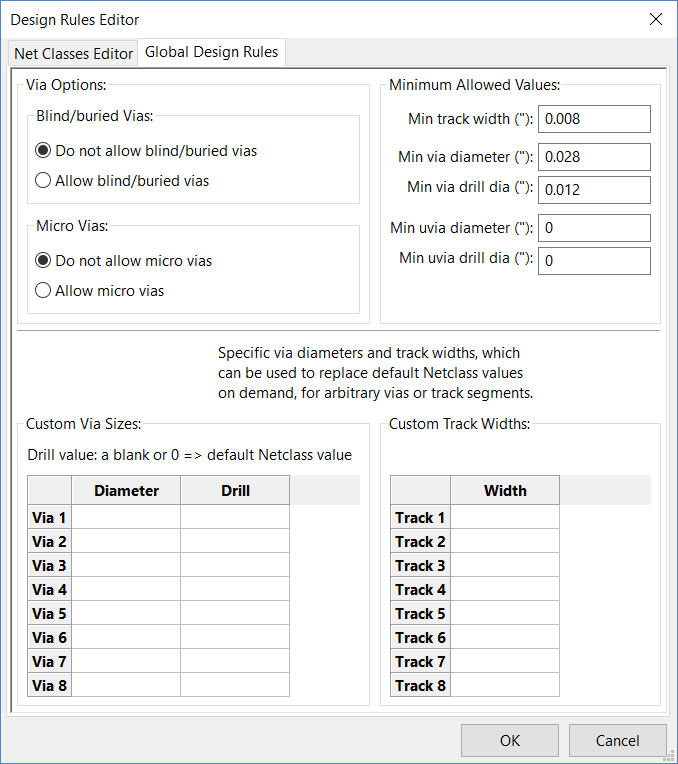
\includegraphics[width=8cm]{Design_rules_2}
    \caption{Reglas de diseño en KiCad}
    \label{fig:Design_rules_general}
  \end{subfigure}
  \caption{Reglas de diseño en KiCad}
  \label{fig:Design_rules}
\end{figure}

 En la figura \ref{fig:Design_rules} se puede observar como las restricciones de diseño anteriomente mencionadas ya se encuentran aplicadas.

\clearpage

\section{Componentes y librerías\label{sec:Componentes_y_librerias}}

Aunque en el esquemático se escogieron los valores de todos los componentes, a la hora de realizar un diseño final hay que tener en cuenta otros muchos parámetros. ¿Qué tamaño tendrá el componente?, ¿cuál será su tolerancia?, ¿qué formato se ajusta mejor, \acrshort{THT} o \acrshort{SMT}? La respuesta a todas estas preguntas acabará definiendo el componente a elegir, su precio y su disponibilidad.

Utilizar componentes en el formato THT puede suponer una ventaja las primeras veces que se realiza una soldadura o al trabajar con electrónica de potencia. En ambos casos se aprovecha el grosor del conector y el hecho de que atraviese la placa para dar mayor comodidad al técnico y disminuir la resistividad de la unión respectivamente. 
\\Por desgracia, al trabajar con electrónica digital o analógica que no involucra alta potencia, la utilización de dichos componentes limita el diseño e impone restricciones que mediante SMT se evitan con relativa facilidad. Un claro ejemplo es la imposibilidad de enrutar pistas bajo los conectores de dichos componentes THT.
\\A lo largo del diseño de la PCB se seleccionará en la medida de lo posible componentes en su formato SMT.

Por simplicidad y comodidad se ha escogido trabajar con una tamaño estándar de 0603 con medidas de 0.063'' x 0.031'' (1,6 mm x 0,8 mm) ya que, por un lado permiten su manejo y soldado sin necesidad de herramientas especiales, y por otro, son medidas muy comunes, facilitándose de esta forma la localización de componentes así como distribuidores primarios y secundarios.

\begin{figure} [h]
    \centering
    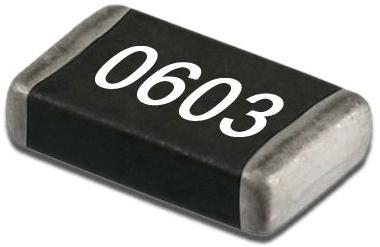
\includegraphics[width=5cm]{0603}
    \caption{Resistencia en formato 0603 \cite{Imagen_0603}}
    \label{fig:0603}
\end{figure}

\subsection{Asignación de footprint\label{sec:Enlazado}}

Tras decidir el tamaño de los componentes ha llegado el momento de enlazar cada uno de los símbolos presentes en el esquemático que se generó al comienzo del proyecto con un componente que contenga un \textit{footprint} y, opcionalmente, un modelo 3D asociado.

Si bien el segundo elemento no es normalmente necesario el primero resulta imprescindible, pues contiene información básica sobre el componente (número de pads y conexiones, tamaño real, serigrafías, etc). 

Como ya se ha mencionado anteriormente, KiCad se caracteriza por tener una gran comunidad que lo respalda. Esto se traduce en que la mayoría de los componentes del mercado ya han sido incluidos en librerías de código abierto disponibles en Internet, lo cual supone un ahorro considerable de tiempo de cara a este o futuros proyectos. 
Por desgracia esto no es siempre suficiente de modo que KiCad ha sido diseñado para, en caso de ser necesario, crear una librería en la que almacenar los \textit{footprints}, serigrafías y modelos 3D que hagan falta, conteniendo las herramientas con las que crear o editar uno ya existente para adaptarlo a las necesidades del proyecto.

\begin{figure} [h]
    \centering
    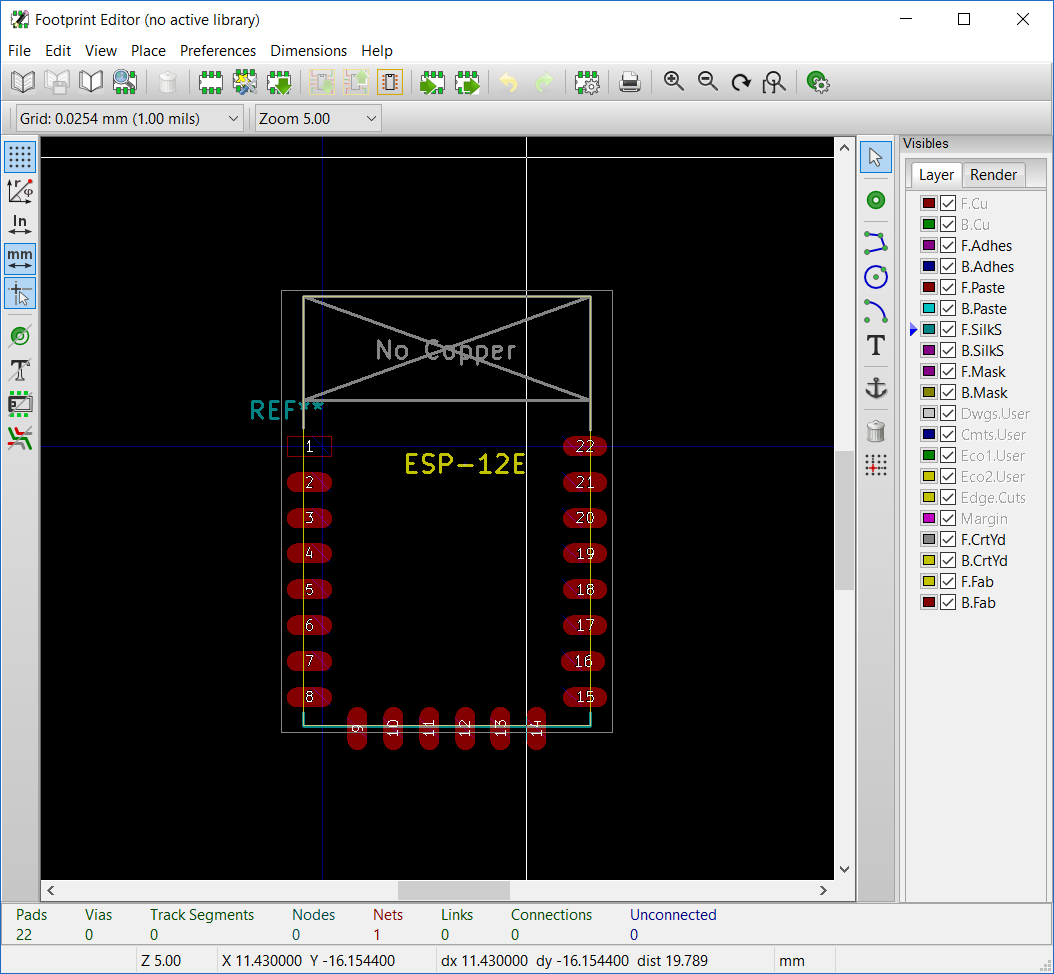
\includegraphics[width=16cm]{Footprint_ESP}
    \caption{\textit{Footprint }modificado para adaptarlo al ESP12-E}
    \label{fig:Footprint_ESP}
\end{figure}

Una vez se han localizado o creado los \textit{footprints} de todos los componentes es necesario asociarlos entre si. Esto permite que en la fase de diseño de la PCB, KiCad pueda cargar una representación física del componente. 
La asociación se realiza con el complemento CvPcb, accesible desde Eeschema. La figura \ref{fig:cvpcb} muestra la interfaz de usuario tras finalizar este proyecto.

\clearpage

A la izquierda aparecen todas las librerías disponibles, en la columna central los componentes de este proyecto y a la derecha los footprints contenidos en la librería seleccionada en la columna izquierda.

\begin{figure} [h]
    \centering
    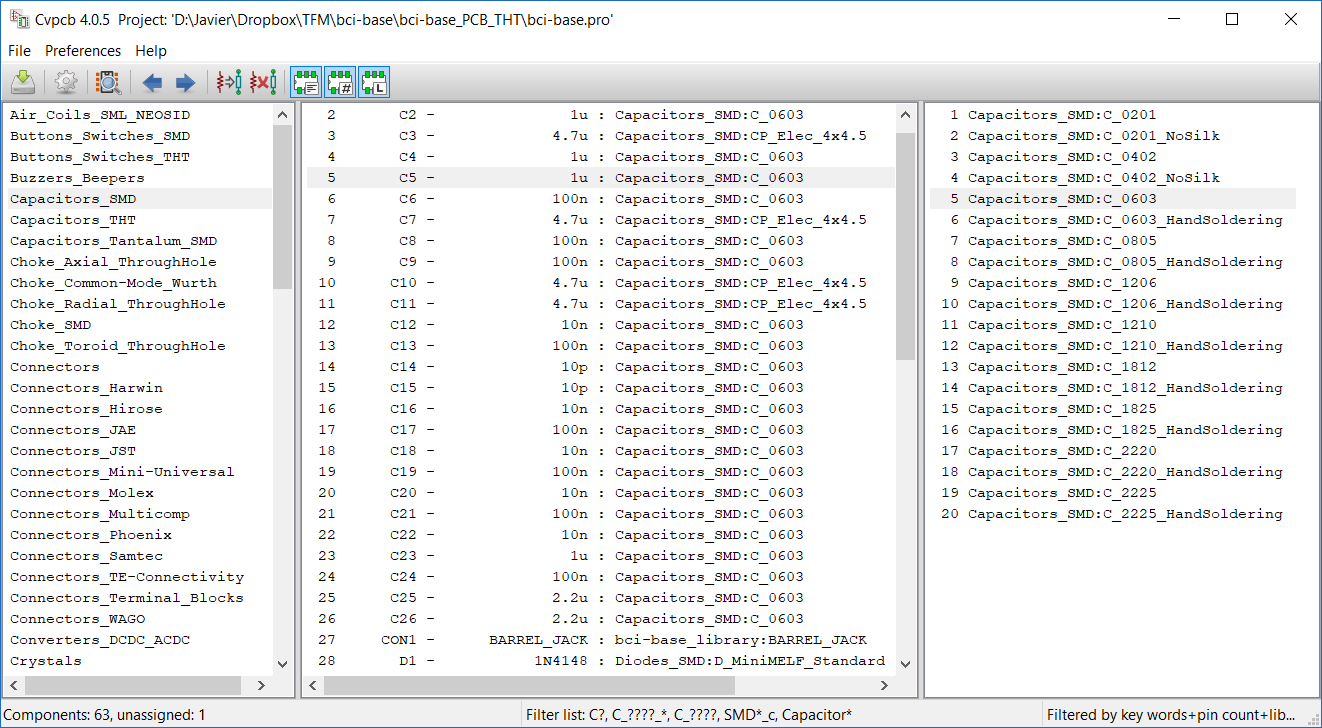
\includegraphics[width=16cm]{cvpcb}
    \caption{Herramienta cvpcb asociando a un componente su \textit{footprint}}
    \label{fig:cvpcb}
\end{figure}

Es posible realizar búsquedas para agilizar el proceso haciendo uso de los tres botones situados en la parte superior derecha. De izquierda a derecha permiten filtrar por palabras clave extraídas del componente, por número de pines y por librería activa.

\clearpage

\section{PCBnew\label{sec:PCBnew}}

Eeschema da como salida dos tipos de archivos que representan la interconexión del los elementos del circuito. Por un lado, un archivo PDF destinado a su lectura por humanos, por otro, un fichero en formato NET. Este último será el fichero de entrada de la herramienta de diseño de PCB denominada PCBnew. 

\begin{figure} [h]
    \centering
    \includegraphics[width=14cm]{pcbnew}
    \caption{Herramienta PCBnew tras finalizar el proyecto}
    \label{fig:pcbnew_1}
\end{figure}

Tras cargar el .net todos los componentes aparecen representados en la zona de trabajo. Cada uno de los conectores muestra una línea que indica a que otros dispositivos se debe conectar para que el la netlist se generada por Eeschema se cumpla.

Para proyectos de menor envergadura como este, la disposición de los elementos se puede realizar de forma manual, pero KiCad está pensado para poder trabajar con diseños de miles de componentes. En estos casos es posible utilizar la propia disposición automática de KiCad o importar la disposición de herramientas externas como FreeRoute.

Una vez todos los componentes se encuentran posicionados, es el momento de conectarlos entre ellos. Con este objetivo se utiliza el trazado de las pistas. Como ya se había mencionado, las características de las pistas vendrán determinadas por las reglas de diseño y el tipo de red al que pertenece (por defecto, de alimentación, de tierra, etc).

Para aquellos puntos comunes a varios dispositivos como son GND o Vcc es posible definir planos. La definición de planos permite, además de ahorrar el trazado de un gran número de pistas, disminuir la resistividad de una conexión, consiguiéndose así que el voltaje sea lo más parecido posible en todo el sistema.
\\La definición de un plano no imposibilita el trazado de una pista que lo atraviese. Todas las pistas que atraviesan un plano son protegidas con una zona de guarda sin cobre que evita cortocircuitos y cuyo grosor viene definido en las reglas de diseño.

En ocasiones será necesario forzar que una parte de la placa no contenga ningún elemento conductor, bien para evitar apantallamientos como en el caso de las antenas, bien para forzar aislamientos entre dos zonas. Para estos casos se puede definir un plano especial denominado ``\textit{keep out area}''. Al contrario que los planos normales, las pistas no pueden atravesarlos.

En ocasiones el propio sistema puede incluir tantos componentes, pistas y planos, que unos elementos acaban afectando a la visibilidad y ocultando otros. Para evitar estos problemas, en la parte derecha hay habilitado un panel que permite activar o desactivar el renderizado de ciertos objetos. Es posible ocultar cualquier grupo de elementos: planos, serigrafías, componentes, etc.
 
\section{Diseño final de la PCB\label{sec:PCB_final}}

El sistema seguido para la disposición de componentes en la PCB ha venido determinado en gran medida por la disposición de componentes en la placa con la que deberá comunicarse. Con el objetivo de minimizar la distancia entre los conectores de ambas placas, la zona encargada de alimentar el sistema ha sido situada en la zona superior izquierda de la placa. La localización del conector que transmitirá las señales a la placa de adquisición también ha sido escogida con esta premisa en mente. Una los elementos más problemáticos han sido situados el resto de los componentes se han posicionado intentando mantener el número de cruces de pistas al mínimo.

\begin{figure} [h]
    \centering
    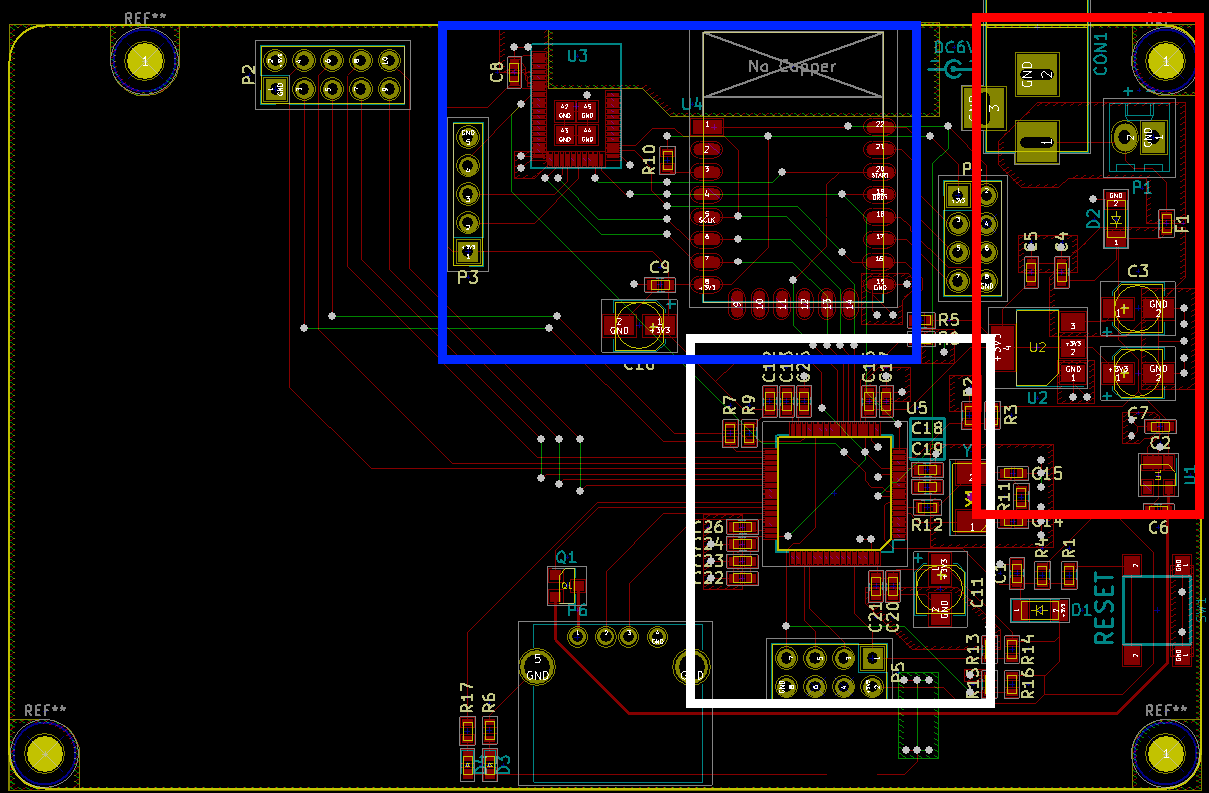
\includegraphics[width=14cm]{Esquema_PCB}
    \caption{Distintas partes que componen la PCB. Alimentación (rojo), microcontrolador (blanco), interfaz inalámbrica (azul).}
    \label{fig:Esquema_PCB}
\end{figure}

En las siguientes secciones se explicará con más detalle cada una de las partes de la PCB, haciendo una división en los tres grandes grupos que la componen: alimentación (rojo), microcontrolador (blanco) e interfaz inalámbrica (azul).

\subsection{Alimentación\label{sec:PCB_alimentacion}}

\subsection{Microcontrolador\label{sec:PCB_alimentacion}}

\subsection{Interfaz inalámbrica\label{sec:PCB_alimentacion}}



	PCB (Añadir BOM)
	
	Primeras pruebas y programación
	
